
\section{Custom Shape Creation}

The purpose of this functionality is to grant the user a simple yet robust shape
structure supporting a set of geometry transformation operations,
so that custom shapes can be modeled with ease. Figure \ref{fig:example} shows an example result.

\begin{figure}[!ht]
	\centering
	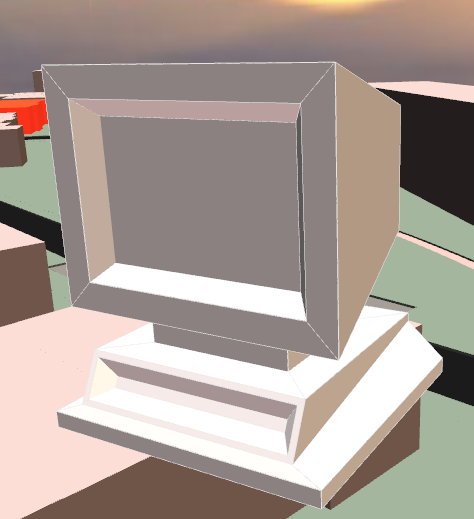
\includegraphics[width=5cm]{gfx/ex-monitor.png}
	\caption{monitor shape modeled in the system}
	\label{fig:example}
\end{figure}

\subsection{Internal Structure}

The defined structure to support the custom shape is based on 4 sided faces.
This decision implies that:
\begin{itemize}
	\item every edge is shared by two faces;
	\item every edge in a face has an opposite edge relating to that face.
\end{itemize}

Besides the \emph{list of vertices} and its positions and the \emph{list of faces}
(each face being a list of 4 vertex indices),
an additional structure is computed: the \emph{edge map}.
It maps which faces share each edge.
This information is used to optimize the low-level operations for
getting the opposite edge and getting the face loop,
a	paramount to the split face loop operation.

Aside from these data structures which hold the shape's form,
there's a \emph{list of face colors}, one for face, to hold the shape's appearance.

These shapes support the undo operation. It was implemented based on the Memento design pattern \cite{despat}.
Each object has an associated stack of states, so the user can return to any previous state of modeling if needed.


\subsubsection{Persistence}

Each modeled object is responsible for saving its geometry data.
The chosen format for persistence was XML and each shape is translated into an XML element.

The format resembles the simplified structure of an OBJ file, but described in XML.
First the vertices are listed -- the order being relevant here -- we assume they start at index 0.
Then each face is defined as an ordered list of 4 vertex indices.
The a list of colors, one for each of the faces described earlier.

\begin{small}
	\begin{verbatim}
	<?xml version="1.0" encoding="utf-8"?>
	  <shape>
	    <vertices count="56">
	      <vertex x="-1" y="-0.627882" z="5.29942"/>
	      ...
	    </vertices>
	  <faces count="54">
	    <face v1="0" v2="1" v3="2" v4="3"/>
	    ...
	  </faces>
	  <colors count="54">
	    <color r="0.9" g="0.9" b="0.9"/>
	    ...
	  </colors>
	</shape>
	\end{verbatim}
\end{small}

\TODO{CLASS HIERARCHY, PROVIDED SHAPES (from CV document)}

\subsubsection{Relevant Algorithms}

\paragraph{Bevel Face}

\begin{figure}[!ht]
    \centering
    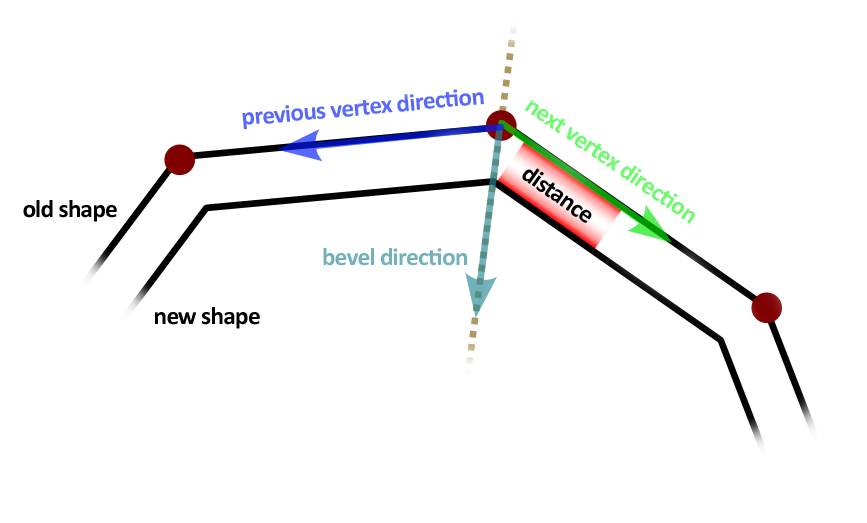
\includegraphics[width=9cm]{gfx/bevel.png}
    \caption{Main directions and relations supporting the bevel operation}
    \label{FIG-GS-BEVEL}
\end{figure}

The algorithm used for beveling faces uses, for each vertex,
the directions from it to the previous and next vertices,
averages it and normalizes it, getting the bevel direction vector with unit length.
The new vertex position is then:

\begin{equation}
	v^{'} = v + b_{dir} \cdot b_{distance}
\end{equation}


\paragraph{Determining Edge Directions}

\begin{figure}[!ht]
    \centering
    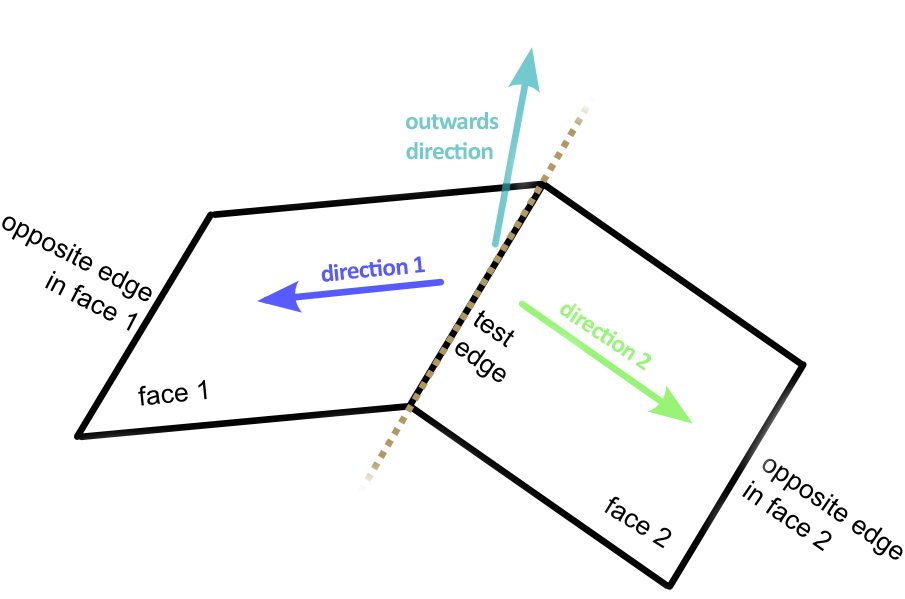
\includegraphics[width=9cm]{gfx/face-dirs.png}
    \caption{Determining edge directions from neighboring faces}
    \label{FIG-GS-FACE-DIRS}
\end{figure}

The most relevant directions according to an edge are those along the faces
which share it and the direction farthest away from the other ones.
 
Calculating direction 1 is easy once the edge map is calculated
and GETOPPOSITEEDGE(EDGE) function defined.

Direction 2 works the same way, this time following the remaining direction.

The outwards direction resembles the concept of a face normal but applied to an edge
-- it points out relating to the neighboring faces.
This direction can be easily found by averaging the face normals
for the faces containing the selected edge.


\subsection{User Interface}

\emph{Face selection} occurs by drawing a stroke exclusively over a face.

\emph{Edge selection} occurs by crossing the desired edge, with the stroke beginning
at one of its neighboring faces and ending on the remaining one.
Figure \ref{fig:selection} illustrates this procedure.

\begin{figure}[!ht]
	\centering
	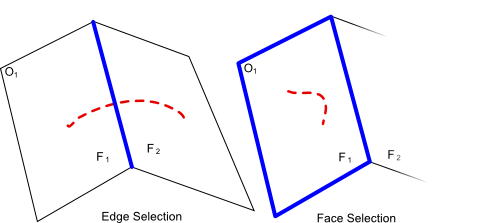
\includegraphics[width=12cm]{gfx/face-edge-selection.png}
	\caption{edge and face selection}
	\label{fig:selection}
\end{figure}

Once the component gets selected, a contextual menu appears in the vicinity
of the selection, allowing the user to select the operation to apply (see figure \ref{fig:contextual}).

\begin{figure}[!ht]
	\centering
	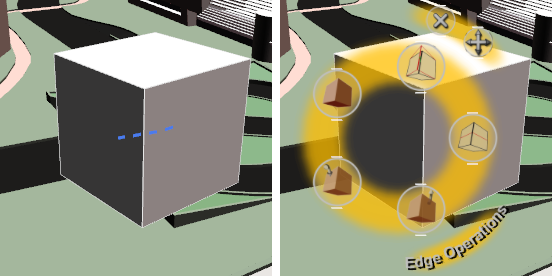
\includegraphics[width=10cm]{gfx/contextual.png}
	\caption{activation of a contextual menu from an edge selection}
	\label{fig:contextual}
\end{figure}

In several of the supported operations one of the parameters is direction.
In those cases the nearest vector direction algorithm is used.
The direction of the ongoing stroke is compared with the set of suggested directions,
with the closest direction being applied in real-time, a mechanism commonly
named \textit{snapping} (see figure \ref{fig:election}).

\begin{figure}[!ht]
	\centering
	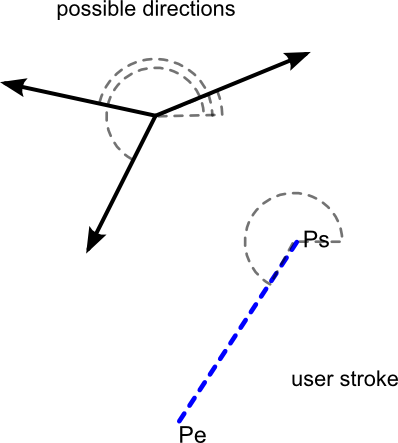
\includegraphics[width=5cm]{gfx/election.png}
	\caption{electing the nearest vector direction}
	\label{fig:election}
\end{figure}

\subsection{Supported Operations}

A description of the supported operations and their provided directions for modification follows,
as seen in figure \ref{fig:shots}

\begin{figure}[!ht]
	\centering
	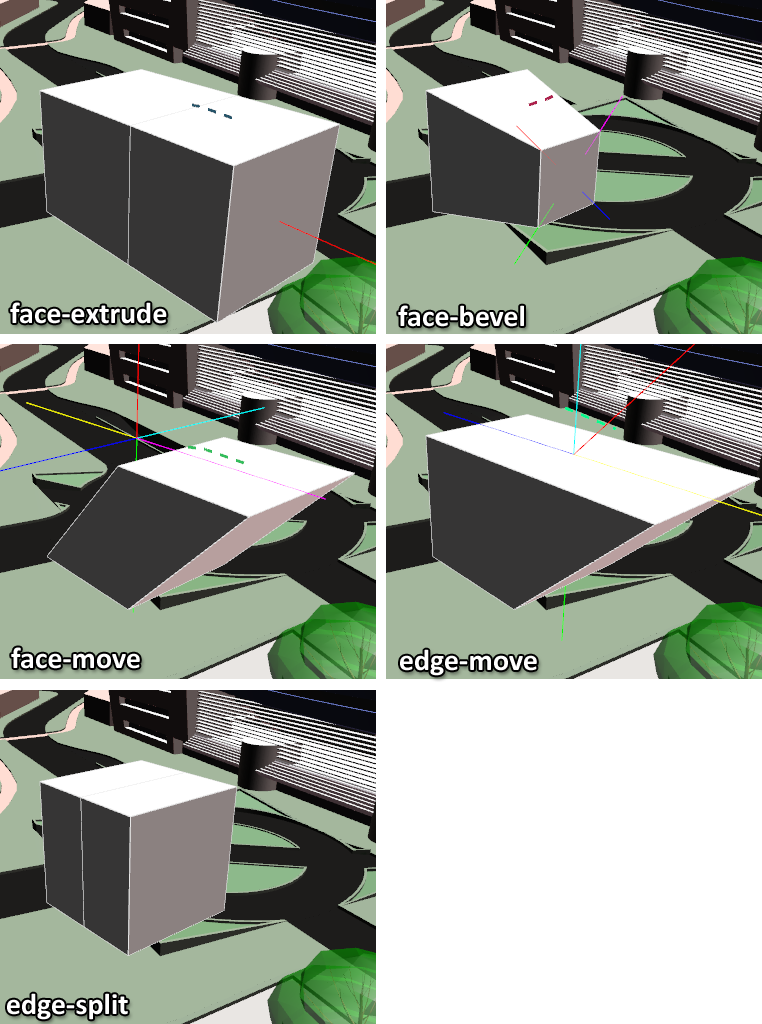
\includegraphics[width=9cm]{gfx/shots2.png}
	\caption{geometry manipulation operations}
	\label{fig:shots}
\end{figure}

\subsubsection{Geometry Manipulation Operations}

\begin{description}
	\item[Face Extrude] --
		the direction is extracted from the select face normal. Displacement based on stroke length.
		
	\item[Face Bevel] --
		the bevel dimension depends on the stroke length.
		
	\item[Face Move] --
		this operation supports not only the normal directions,
		but also the directions from the face center towards the four boundary edges.
		
	\item[Edge Move] --
		supports the edge normals along with the directions towards the neighboring faces.
		
	\item[Edge Split] --
		this operation occurs immediately since it doesn't require any real-time input from the user.
		The sketched cut propagates throughout the intrinsic selected face loop, each edge cutting
		the opposite edge in each face of the loop, until either no more faces occur or an already
		visited face is revisited.
\end{description}

\subsubsection{Other Operations}

\begin{description}
	\item[Undo] --
		any shape operation previously defined can be reverted.
		
	\item[Loading and Saving] --
		the object can be loaded from or saved to the XML format defined above.
		Exporting content from an external 3D modeler is straightforward.
		An exporting plug-in for Blender was implemented in Python.
\end{description}

